\documentclass[t, aspectratio=169, dvipdfmx]{beamer}

\usepackage{url}
\usepackage{hyperref, pxjahyper}
\usepackage{cite}
\usepackage{graphicx}
\usepackage{amsmath, amssymb}
\usepackage{tcolorbox, xcolor}
\usepackage{multicol}
\usepackage{tikz}

\setbeamertemplate{navigation symbols}{}
\usetheme{AnnArbor}
\usecolortheme{beaver}
\usefonttheme{professionalfonts}

\setbeamertemplate{items}[default]
\setbeamercolor{structure}{fg=darkred}
\setbeamercolor{block title}{fg=white, bg=darkred}
\setbeamercolor{block body}{fg=black, bg=red!10}

\tcbuselibrary{skins}
\newtcolorbox{term}[1]{enhanced,
  title={#1},
  fonttitle=\gtfamily\small,
  frame style={left color=orange, right color=red},
  colback=orange!10,
  coltitle=white,
  top=0mm, bottom=0mm,
  before upper={\setbeamercolor{structure}{fg=orange}}
  }
\newtcolorbox{mytheorem}[1][定理]{enhanced,
  title={#1},
  fonttitle=\gtfamily\small,
  frame style={left color=pink, right color=red},
  colback=red!10,
  coltitle=white,
  top=0mm, bottom=0mm,
  before upper={\setbeamercolor{structure}{fg=yellow}}
  }

\newcommand{\comb}[2]{{}_{#1}\mathrm{C}_{#2}}
\newcommand{\perm}[2]{{}_{#1}\mathrm{P}_{#2}}

\hypersetup{
  colorlinks=true,
}

\title[競プロ体験会]{競技プログラミングを始めよう}
\author{終に鮭}
\institute[OUCRC]{電子計算機研究会}
\date[12/2]{December 2, 2020}

\begin{document}
\frame{\titlepage}

\begin{frame}
  \frametitle{自己紹介}
  \begin{itemize}
    \item 終に鮭
    \item 情報系学科1回生
    \item 競プロ歴8ヶ月(最初のコンテストは4/4のABC161)
    \begin{itemize}
      \item AtCoderしかやってない
      \item 現在のレートは\textcolor{green!50!black}{877}
      \item ごくまれにyukicoderの問題も解く
    \end{itemize}
    \item プログラミング歴は4~5年(?)
    \begin{itemize}
      \item 現在メインで使っている言語はPython, C++, JavaScript
      \item 使ったことのある言語はC, Java, Visual Basic, PHP
    \end{itemize}
  \end{itemize}
\end{frame}

\begin{frame}
  \frametitle{今日の内容}
  \begin{multicols}{2}
    \tableofcontents
  \end{multicols}
\end{frame}

\section{競技プログラミングとは?}
\frame{\sectionpage}

\begin{frame}[c]
  \frametitle{競技プログラミングとは}
  \center{\huge プログラミング早解きコンテストのこと!!}
\end{frame}

\subsection{競プロのいいところ}
\begin{frame}
  \frametitle{競プロのいいところ}
  \begin{itemize}
    \item プログラムが書けるようになる
    \begin{itemize}
      \item 化生の友人(未経験)にAtCoderを教えたらプログラミング1が楽単になった
    \end{itemize}
    \item アルゴリズム・データ構造を学べる
    \begin{itemize}
      \item 次回があればこの部分を掘り下げて勉強会を開くかも
    \end{itemize}
    \item 計算量を意識して書くようになる
    \begin{itemize}
      \item 逆に、$1 \leq N \leq 10^6$なら$O(N \log N)$で2秒に間に合うな、とメタ読みできる
    \end{itemize}
    \item 数学力がつく
    \item 就活に役立つことがある(らしい)
    \begin{itemize}
      \item レートが実力の証明になる
    \end{itemize}
  \end{itemize}
\end{frame}

\subsection{コンテストの形式}
\begin{frame}
  \frametitle{コンテストの形式}
  参加者全員に同じ課題が与えられ、より早く要求を満たすプログラムを記述することを競う
  \begin{itemize}
    \item \textcolor{red}{アルゴ:短時間、最適解が出せる}
    \item マラソン:中長時間、最適解を目指す
    \item コードゴルフ:より短いコードを記述することを競う
  \end{itemize}
\end{frame}

\subsection{オンラインジャッジ}
\begin{frame}
  \frametitle{オンラインジャッジ}
  \begin{itemize}
    \item \textcolor{red}{\href{https://atcoder.jp/home}{AtCoder}(日本):週1,2回、全問日本語に対応}
    \item \href{http://codeforces.com/}{CodeForces}(ロシア):開催頻度がすごい
    \item \href{https://www.tc3.co.jp/topcodersrm/}{TopCoder}(アメリカ):マラソンが充実してる
    \item \href{http://judge.u-aizu.ac.jp/onlinejudge/}{Aizu Online Judge}(日本):\href{https://www.ioi-jp.org/}{JOI}や\href{https://icpc.iisf.or.jp/}{ICPC}の過去問が解ける
  \end{itemize}
\end{frame}

\section{AtCoderをやってみよう}
\frame{\sectionpage}

\subsection{対応言語}
\begin{frame}
  \frametitle{対応言語}
  多すぎて \TeX がクラッシュするので一部のみ抜粋(独断で選びました)
  \begin{block}{主な対応言語(ABC183時点)}
    \begin{multicols}{2}
      \begin{itemize}
        \item C / C++
        \item Java
        \item C\#
        \item Rust
        \item Python / PyPy
        \item Cython
        \item JavaScript (Node.js)
        \item PHP
        \item Ruby
        \item Perl
      \end{itemize}
    \end{multicols}
    延べ57言語が使用可能
    \footnote{\url{https://atcoder.jp/contests/abc182/rules}}
  \end{block}
\end{frame}

\subsection{書き方と注意点}
\begin{frame}[containsverbatim]
  \frametitle{プログラムの書き方と注意点}
  \begin{itemize}
    \item 「入力」は標準入力から受け取れる、「出力」は標準出力に出す
    \begin{itemize}
      \item コマンドライン引数は使わない
      \item 標準入出力を備えていない言語の場合はちょっと特殊(practice contest参照)
      \item 例えばJavaScriptでは \verb|/dev/stdin| からファイル入力、\verb|console.log| で出力
    \end{itemize}
    \item (B問題ぐらいから)制約に注意する
    \begin{itemize}
      \item 算術オーバーフロー
      \begin{itemize}
        \item 黒魔法 \verb|#define int long long|
      \end{itemize}
      \item 実行時間制限超過(TLE:Time Limit Exceeded)
      \begin{itemize}
        \item 1秒間に処理できる量は$10^7$から$10^8$ステップ程度
      \end{itemize}
      \item スタックオーバーフロー
      \begin{itemize}
        \item 再帰の制限は緩められる場合がある
      \end{itemize}
      \item \verb|out_of_range|
    \end{itemize}
  \end{itemize}
\end{frame}

\subsection{提出の練習}
\begin{frame}
  \frametitle{提出の練習}
  \begin{itemize}
    \item 常設中のコンテストから\href{https://atcoder.jp/contests/practice}{practice contest}に飛ぶ
    \item 問題タブから「A - Welcome to AtCoder」を選んで解いてみよう
    \begin{itemize}
      \item 自前のエディタで書くのがおすすめ
      \item 事前調査で回答いただいた言語のサンプルを\href{https://github.com/AAAR-Salmon/procon/tree/main/introduction/sample_practice}{ここ}に用意してあります
    \end{itemize}
  \end{itemize}
  \begin{figure}[b]
    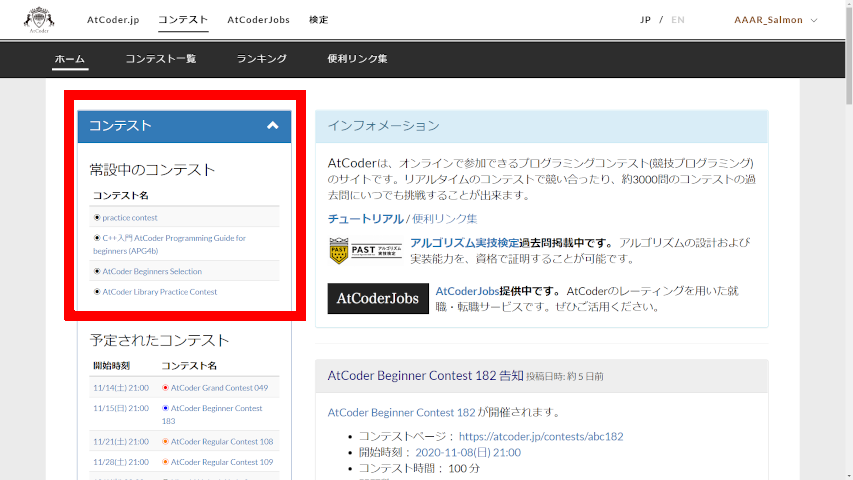
\includegraphics[height=110pt]{atcoder_home.png}
    \caption{AtCoderのコンテストトップページ}
    \label{practice_contest}
  \end{figure}
\end{frame}

\begin{frame}
  \frametitle{提出の練習}
  \begin{itemize}
    \item \textcolor{red}{必ずコードテストする}
    \begin{itemize}
      \item 手元の実行環境を使う
      \item AtCoderのコードテスト機能を使う
    \end{itemize}
    \item 問題ページ下部から提出
  \end{itemize}
\end{frame}

\subsection{典型問題を解いてみよう}
\begin{frame}
  \frametitle{「いかにも競プロ」な問題を解いてみよう}
  \begin{itemize}
    \item どんな問題?
    \begin{itemize}
      \item 文字列操作系問題
      \item 数学の問題
      \begin{itemize}
        \item 小数の計算、幾何、方程式、数え上げ
      \end{itemize}
      \item データ構造を活かす問題
      \begin{itemize}
        \item 配列、集合、スタック・キュー、Union-Find、全域木
      \end{itemize}
      \item 典型アルゴリズムを使う問題
      \begin{itemize}
        \item ソート、探索、累積和、しゃくとり法、いもす法、動的計画法、貪欲法、最短経路問題、最大流問題
      \end{itemize}
    \end{itemize}
  \end{itemize}
\end{frame}

\begin{frame}
  \frametitle{初心者におすすめの問題}
  \begin{itemize}
    \item \href{https://kenkoooo.com/atcoder}{AtCoder Problems}(有志サイト)にバーチャルコンテストを用意したのでやってみよう
    \item 制限時間は1時間
    \item 全問解ききることは想定していないので解けそうな問題から解いてください
    \item インターネットや本で調べてもOK
    \item 全問解説すると時間がかかるので、全員解けた問題と聞いても誰もわからなさそうな問題は解説しません
  \end{itemize}
\end{frame}

\subsection{解説}
\begin{frame}[c]
  \frametitle{解説}
  \center{\huge 解説を始めます}
\end{frame}

\begin{frame}
  \frametitle{配点基準}
  \begin{table}[t]
    \caption{今回採用した配点の基準}
    \begin{tabular}{ccc}\hline
      配点 & 問題数 & 問題の要素 \\ \hline
      50 & 3 & \begin{tabular}{c}
        if文のみで解ける \\
        数学的考察が不要
      \end{tabular} \\ \hline
      100 & 4 & \begin{tabular}{c}
        if文のみで解けるが、場合分けが難しい \\
        文字列操作が必要 \\
        簡単な数学的要素が含まれる
      \end{tabular} \\ \hline
      200 & 7 & \begin{tabular}{c}
        配列を扱う \\
        ループまたは再帰関数が必要 \\
        単純な多重ループが必要 \\
        小数を扱う \\
        数学的考察が含まれる
      \end{tabular} \\ \hline
    \end{tabular}
  \end{table}
\end{frame}

\begin{frame}
  \frametitle{配点基準}
  \begin{table}[t]
    \caption{今回採用した配点の基準}
    \begin{tabular}{ccc}\hline
      配点 & 問題数 & 問題の要素 \\ \hline
      300 & 3 & \begin{tabular}{c}
        ナイーブな実装が通用しない \\
        コーナーケースへの対応が必要
      \end{tabular} \\ \hline
      400 & 3 & \begin{tabular}{c}
        特殊なデータ構造を用いる \\
        比較的複雑な典型アルゴリズムを用いる \\
        $\mod 10^9+7,998244353$ \\
        複合的なスキルが必要
      \end{tabular} \\ \hline
    \end{tabular}
  \end{table}
\end{frame}

\begin{frame}[c]
  \center{\huge 50点問題}
\end{frame}
\begin{frame}[containsverbatim]
  \frametitle{ABC Swap}
  \begin{table}
    \caption{箱とその中身}
    \begin{minipage}{0.3\hsize}
      \begin{center}
        \begin{tabular}{|c|c|c|} \hline
          A & X \\ \hline
          B & Y \\ \hline
          C & Z \\ \hline
        \end{tabular}
      \end{center}
    \end{minipage}
    \begin{minipage}{0.3\hsize}
      \begin{center}
        \begin{tabular}{|c|c|c|} \hline
          A & \textcolor{red}{Y} \\ \hline
          B & \textcolor{red}{X} \\ \hline
          C & Z \\ \hline
        \end{tabular}
      \end{center}
    \end{minipage}
    \begin{minipage}{0.3\hsize}
      \begin{center}
        \begin{tabular}{|c|c|c|} \hline
          A & \textcolor{red}{Z} \\ \hline
          B & X \\ \hline
          C & \textcolor{red}{Y} \\ \hline
        \end{tabular}
      \end{center}
    \end{minipage}
  \end{table}
  箱 $A,B,C$ の中身 $X,Y,Z$ について、$A$ と $B$、$A$ と $C$ を順に入れ替えたときの中身を求めよ
  \begin{itemize}
    \item \verb|swap| 関数を使ってシミュレーションする
    \item 順番を決め打ちして出力する
  \end{itemize}
\end{frame}

\begin{frame}[containsverbatim]
  \frametitle{AC or WA / Sheep and Wolves}
  それぞれ $N=M$ か、$W \geq S$ か判定せよ
  \begin{itemize}
    \item 条件演算子 \verb|cond ? a : b| を使うと短く書ける
  \end{itemize}
\end{frame}

\begin{frame}[c]
  \center{\huge 100点問題}
\end{frame}

\begin{frame}[containsverbatim]
  \frametitle{Accepted...?}
  長さ6の文字列 $S$ に \verb|'1'| はいくつ含まれるか
  \begin{itemize}
    \item 6回if文書く卍
    \item for文を回す
    \begin{itemize}
      \item 文字列のまま判別(おすすめ)
      \begin{itemize}
        \item 範囲for文でもよい
      \end{itemize}
      \item 10進整数の各桁を判別
    \end{itemize}
    \item \verb|count_if| のような関数を使う
    \begin{itemize}
      \item イテレータとラムダ式の知識を要するので初心者にはおすすめしない
    \end{itemize}
  \end{itemize}
\end{frame}

\begin{frame}[containsverbatim]
  \frametitle{Repeat ACL}
  文字列 \verb|ACL| を $K$ 回繰り返した文字列を出力せよ
  \begin{itemize}
    \item 5回if文書く卍
    \item $K$ 回 \verb|"ACL"| を出力する
    \item 空文字列に $K$ 回 \verb|"ACL"| を連結した文字列を出力する
    \begin{itemize}
      \item Pythonでは \verb|'ACL' * K| でよい
    \end{itemize}
  \end{itemize}
\end{frame}

\begin{frame}[containsverbatim]
  \frametitle{CODE FESTIVAL 2015}
  文字列の末尾の \verb|2014| を \verb|2015| に置き換えよ
  \begin{itemize}
    \item 末尾4文字が \verb|'2014'| であることが確定しているので、末尾1文字を \verb|'5'| に書き換えれば良い
    \begin{itemize}
      \item C++の場合末尾1文字は \verb|S[S.length() - 1]|
      \item 文字列をスタック的に扱って \verb|S.pop_back(); S.push_back('5');| するという方法もある
    \end{itemize}
  \end{itemize}
\end{frame}

\begin{frame}
  \frametitle{Number of Multiples}
  \begin{figure}[b]
    \begin{tabular}{*{13}{|c}|} \hline
      1 & 2 & 3 & 4 & 5 & 6 & 7 & 8 & 9 & 10 & 11 & 12 & $\cdots$ \\ \hline
    \end{tabular}
    \caption{自然数の列}
  \end{figure}
  $[L,R]$ の範囲にいくつ $d$ の倍数があるか
  \begin{itemize}
    \item $L,R,d$ から計算(時間計算量 $O(1)$)
    \begin{itemize}
      \item $L$ 以上の最小の $d$ の倍数は $\lceil L/d \rceil \times d=\lfloor (L+d-1)/d \rfloor \times d$
      \item $R$ 以下の最大の $d$ の倍数は $\lfloor R/d \rfloor \times d$
      \item 求める数は $\lfloor R/d \rfloor - \lfloor (L+d-1)/d \rfloor + 1$
    \end{itemize}
    \item $i(L \leq i \leq R)$ について、$d$ の倍数か判定($O(R-L)$)
    \item $d$ の倍数 $n=di(1 \leq n \leq 100)$ について、 $L \leq n \leq R$ か判定($O(\frac{1}{d})$)
  \end{itemize}
\end{frame}

\begin{frame}[c]
  \center{\huge 200点問題}
\end{frame}

\begin{frame}
  \frametitle{Fourtune Cookies}
  $A,B,C,D$ を2つグループに分けて、それぞれの総和が等しくなることがあるか
  \begin{itemize}
    \item $A \leq B \leq C \leq D$ としても一般性を失わない(これはソートすれば簡単に得られる)
    \begin{itemize}
      \item 食べるクッキーと残るクッキーの美味しさの総和が等しくなることがある \\
      $\iff$ $A+D=B+C$ or $D=A+B+C$
    \end{itemize}
    \item bit全探索で食べるクッキーと食べないクッキーの全ての組み合わせを検証する
    \begin{itemize}
      \item 4要素なので組み合わせは $2^4=16$ 通りだけ
    \end{itemize}
  \end{itemize}
\end{frame}

\begin{frame}
  \frametitle{天下一プログラマーコンテスト1998}
  $a_0=100,a_1=100,a_2=200,a_{n}=a_{n-1}+a_{n-2}+a_{n-3}$ が与えられるので $a_{19}$ を計算せよ
  \begin{itemize}
    \item いわゆる動的計画法(DP:Dynamic Programming)を使う
    \begin{term}{動的計画法}
      \begin{itemize}
        \item 帰納的な関係を利用
        \item 部分問題の計算結果を記録
      \end{itemize}
    \end{term}
    \begin{itemize}
      \item 配列を使って $a[i]=a[i-3]+a[i-2]+a[i-1]$ を $i=3,\ldots,19$ でやって $a[19]$ を求める
    \end{itemize}
    \item 再帰関数を使う
    \begin{itemize}
      \item $f(0)=100, f(1)=100, f(2)=200, f(n)=f(n-1)+f(n-2)+f(n-3)$ として $f(19)$ を実行
      \item ただし適切にメモ化などを行わないと69748回の関数呼び出しが行われてよくない
    \end{itemize}
    \item 手計算しておいて出力卍
  \end{itemize}
\end{frame}

\begin{frame}
  \frametitle{Addition}
  偶奇が等しい2数を足し合わせていき、最後に1つだけ残るか
  \begin{itemize}
    \item 偶奇が等しいかつそのときに限り、2数の和は偶数である
    \item 黒板に数が1つだけ残ることは以下に同値である
    \begin{itemize}
      \item $\sum A_i$ が偶数
      \begin{itemize}
        \item オーバーフローに注意
      \end{itemize}
      \item $A_i$ のうち、奇数が偶数個だけ存在する
    \end{itemize}
  \end{itemize}
\end{frame}

\begin{frame}
  \frametitle{Product Max}
  $a \leq x \leq b, c \leq y \leq d$ のときの $xy$ の 最大値を求めよ
  \begin{table}[t]
    \caption{$a,b$の範囲に対する$\max(xy)$}
    $$\begin{array}{|c||c|c|c|} \hline
      & 0 \leq c \leq d & c \leq 0 \leq d & c \leq d \leq 0 \\ \hline\hline
      0 \leq a \leq b & bd & bd & ad \\ \hline
      a \leq 0 \leq b & bd & \max(ac,bd) & ac \\ \hline
      a \leq b \leq 0 & bc & ac & ac \\ \hline
    \end{array}$$
  \end{table}
  \begin{itemize}
    \item いずれにせよ $\max(ac,ad,bc,bd)$ をとればよい
  \end{itemize}
\end{frame}

\begin{frame}[containsverbatim]
  \frametitle{高橋くんと文字列操作}
  回転を繰り返して所定の文字列が得られるか
  \begin{itemize}
    \item 回転、循環シフト(rotation, circular shift)と言われる操作
    \begin{term}{回転、循環シフト}
      \begin{itemize}
        \item ビット列、配列またはキューの先頭または末尾の要素を、末尾または先頭へ移動する操作
      \end{itemize}
    \end{term}
    \begin{itemize}
      \item C++では \verb|algorithm| ヘッダ内の \verb|rotate| 関数で実現できる
      \item Pythonでは \verb|str.rotate| メソッドで実現できる
    \end{itemize}
    \item $|s|$ 回の操作で元の文字列に戻る
    \item 回転の計算量が $O(|s|)$ 、文字列比較の計算量が $O(|s|)$ ならば全体の時間計算量は $O(|s|^2)$
    \item $s+s$ の $[|s|-i, 2|s|-i)$ の範囲を取り出しても $i$ 回操作したのと同じ文字列が得られる
  \end{itemize}
\end{frame}

\begin{frame}[containsverbatim]
  \frametitle{Magic 2}
  $A,B,C$ のうちいずれかを2倍する操作を $K$ 回まで繰り返し、$A<B<C$ にすることができるか
  \begin{itemize}
    \item $A < 2^b B < 2^c C (b+c \leq K)$ なる $b,c$ が存在すればよい
    \begin{itemize}
      \item $K$ 回のループの間に、$A<B$ となるまで \verb|B *= 2| をし、$A<B$ になったら \verb|C *= 2| する
      \item $A<B<C$ ならば成功、そうでなければ失敗
    \end{itemize}
  \end{itemize}
\end{frame}

\begin{frame}[containsverbatim]
  \frametitle{Takahashikun, The Strider}
  1m進みその場で $X$ 度回転することを繰り返したとき、何回目で元の位置に戻るかを求めよ
  \begin{itemize}
    \item 高橋くんは円周上を移動するから、$KX$ が360の倍数となるような最小の $K$ を求める
    \item $X,360$ の最小公倍数を $l$ 、最大公約数を $g$ とすると、$KX=l, lg=360X$ より $K=360/g$
    \item 最小公倍数を求める関数はたいてい用意されているし、ユークリッドの互除法で簡単に実装できる
    \item もちろん、\verb|X*i| が360の倍数になるかを順に判定してもよい
  \end{itemize}
\end{frame}

\begin{frame}[c]
  \center{\huge 300点問題}
\end{frame}

\begin{frame}[containsverbatim]
  \frametitle{Connection and Disconnection}
  $S$ を $K$ 回繰り返した文字列について、最小で何文字置き換えればどの隣り合う2文字も相異なるようにできるか
  \begin{itemize}
    \item $K$ が最大で $10^9$ になるので、愚直にシミュレートできない
    \item $T$ は $S$ を $K$ 回繰り返したものなので $S$ についての解を $K$ 倍する
    \begin{itemize}
      \item ただし $S$ の始端と終端が同じである場合は注意が必要
      \begin{itemize}
        \item $S$ の両端を除いた部分が $K$ 回、始端と終端が各1回、$S$ の終端と $S$ の始端のつなぎ目が $K-1$ 回出る
      \end{itemize}
      \item $S$ が全て同じ文字で構成される場合も分ける必要がある
    \end{itemize}
    \begin{figure}[b]
      \caption{$S$ の始端と終端が同じである場合の $T$ の例}
        \begin{center}\tt
          aaa b cccc ddddd eee aaa|aaa b cccc ddddd eee aaa \\
          aza b czcz dzdzd eze aza|zaz b czcz dzdzd eze aza
        \end{center}
    \end{figure}
  \end{itemize}
\end{frame}

\begin{frame}[containsverbatim]
  \frametitle{DNA Sequence}
  \verb|A,T,C,G| からなる文字列 $S$ の連続する空でない部分文字列 $T$ について、\verb|A| と \verb|T|、\verb|C| と \verb|G|の数が等しいものの数を求めよ
  \begin{itemize}
    \item $N \leq 5000$ より $\comb{N}{2}(<2 \times 10^7)$ 通りを全探索しても間に合う
    \begin{itemize}
      \item ただし判定を $O(1)$ でする必要がある
      \item $S$ の $[0,n)$ の範囲に含まれる \verb|A,T,C,G| の個数をあらかじめ $O(N)$ でカウントしておけば $[a,b)$ の範囲でも $O(1)$ で求められる
    \end{itemize}
    \item 余談:Pythonは配列の処理がめちゃくちゃ遅いのでPyPyを使わないと通りませんでした
    \begin{itemize}
      \item NumPyなら通るかも
    \end{itemize}
  \end{itemize}
\end{frame}

\begin{frame}[containsverbatim]
  \frametitle{One Quadrillion and One Dalmatians}
  名前が順に \verb|a,b,...,z,aa,ab,...,az,...,za,...,zz,aaa,...| となるとき、$N$ 番目の名前を求めよ
  \begin{itemize}
    \item 一見10進数を26進数に変換する問題に見える
    \item \verb|a| と \verb|aa| は異なる
    \begin{itemize}
      \item \verb|a, aa, aaa| はそれぞれ1,2,3桁の1番目なので先に名前の長さを求めれば26進数への変換に持ち込める
    \end{itemize}
    \item 名前が $L$ 文字である条件は
    $$\sum_{i=0}^{L-1}26^i \leq N < \sum_{i=0}^{L}26^i$$
    であるから、$N - \sum_{i=0}^{L-1}26^i$を26進数へ変換すればよい
  \end{itemize}
\end{frame}

\begin{frame}[c]
  \center{\huge 400点問題}
\end{frame}

\begin{frame}
  \frametitle{Connect Cities}
  すべての都市を相互に移動できるようにするには最小で何本の道路を新しく作ればよいか
  \begin{itemize}
    \item Union-Findを使う典型問題
    \begin{term}{Union-Find(Disjoint-set Data Structure)、素集合データ構造}
      \begin{itemize}
        \item UnionとFindの操作が定義されている集合族データ型
        \item Union(Merge): 2つの集合をまとめて1つにする
        \item Find: ある要素がどの集合に含まれるかを探索し、代表元を返す
        \item しばしば森(閉路を持たないグラフ、木の集合)として表現される
      \end{itemize}
    \end{term}
    \item $\{0\},\ldots,\{N-1\}$ の $N$ 個の集合を持ったUnion-Findを生成する
    \item 各道路についてUnionして、最終的なグループ数 $g$ を求める。解は $N-g$
  \end{itemize}
\end{frame}

\begin{frame}
  \frametitle{Union-Find森}
  \usetikzlibrary{graphs}
  \tikzstyle{every node}=[circle, draw]
  \tikz[baseline=0pt]
    \node{0}
      child{node{1}}
      child{node{2}
        child{node{3}}
        child{node{4}}
      };
  \tikz[baseline=0pt]
    \node{5};
  \tikz[baseline=0pt]
    \node{6}
      child{node{7}
        child{node{8}}
      };
  \tikz[baseline=43pt, font=\small, every node/.style={draw=none}]
    \draw[->] (0,0) -- (2,0) node[midway, above] {merge(3,8)};
  \tikz[baseline=0pt]
    \node{0}
      child{node{1}}
      child{node{2}
        child{node{4}}
      }
      child{node{3}
        child{node{6}
          child{node{7}}
          child{node{8}}
        }
      };
  \tikz[baseline=0pt]
    \node{5};
\end{frame}

\begin{frame}
  \frametitle{Div Game}
  整数 $N$ は相異なる素数の冪で何回割り切ることができるか
  \begin{itemize}
    \item 素因数分解すれば簡単に解ける
    \begin{itemize}
      \item $N=p_{1}^{e_{1}} p_{2}^{e_{2}} \cdots p_{n}^{e_{n}} (i \neq j \implies p_{i} \neq p_{j})$ で表されるとき、$e_i \geq \sum_{k=1}^{a_i}k$ を満たす最大の $a_i$ についてその和を求めればよい
    \end{itemize}
    \item $N \leq 10^{12}$ であるから、$[2,N]$ の範囲を試し割りすることはできない
    \begin{mytheorem}
      自然数 $N \geq 2$ について、$N$ が素数でない $\iff$ $N$ は $\sqrt{N}$ 以下の素因数を持つ
    \end{mytheorem}
    \item 素因数は疎であるから、連想配列に格納するとよい
    \begin{itemize}
      \item $p_i$ は再利用しないので $e_i$ のみ配列に格納しておいても十分
    \end{itemize}
  \end{itemize}
\end{frame}

\begin{frame}
  \frametitle{Redistribution}
  総和が $S$ で全ての項が3以上である数列はいくつ存在するか。$10^9+7$で割ったあまりを求めよ
  \begin{itemize}
    \item 条件を満たす数列の項数 $N$ の範囲は $1 \leq N \leq S/3$
    \begin{itemize}
      \item \underline{項数 $N$ の数列 $(a_n)$ について}、条件は次のように言い換えられる
      \begin{tcolorbox}
        $a_i \geq 0, a_1+\cdots+a_N=S-3N$
      \end{tcolorbox}
      \item このような条件を見たす数列は $S-3N$ 個の $\circ$ と $N-1$ 本の $|$ の並びに対応し、その場合の数は $\perm{S-2N-1}{S-3N}/(N-1)!$
      \item 順列は大きな数になるから途中であまりを取る必要がある
      \item 割り算がとてもめんどくさい(モジュラ逆数を求めるには冪を求める必要がある)
      \begin{itemize}
        \item フェルマーの小定理を用いて $x/y = xy^{-1} \equiv xy^{p-2} \mod p$
        \begin{mytheorem}[フェルマーの小定理]
          $a$ と $p$ が互いに素であるとき、$a^{p-1} \equiv 1 \mod p$
        \end{mytheorem}
      \end{itemize}
    \end{itemize}
  \end{itemize}
\end{frame}

\begin{frame}
  \frametitle{Redistribution}
  \begin{itemize}
    \item DPを使うことで順列の計算を回避できる
    \begin{itemize}
      \item 総和が $S$ となるようなすべての項が3以上である\underline{空でもよい}数列の場合の数を $A[S]$ とおく
      \begin{itemize}
        \item すなわち解は $A[S]$
        \item 空な数列()の和は0であるから $A[0]=1$
      \end{itemize}
      \item 総和 $i-3$ で条件(各項が3以上)を満たす数列について考える
      \begin{itemize}
        \item この数列の末尾に3を加えると、総和 $i$ で条件を満たす新たな数列が生成できる
      \end{itemize}
      \item 総和 $i-4,\ldots,0$ で条件を満たす数列の末尾に $4,\ldots,i+3$ を加えても同様に総和 $i$ で条件を満たす
      \item 以上より $A[i]=A[i-3]+A[i-4]+\cdots+A[0],A[2]=A[1]=0,A[0]=1$
      \begin{itemize}
        \item 遷移が $O(S)$、各項の計算量が $O(S)$ であるから計算量は $O(S^2)$
      \end{itemize}
      \item $A[i-1]=A[i-4]+\cdots+A[0]$ より、$A[i]=A[i-3]+A[i-1]$ に変形できる
      \begin{itemize}
        \item この場合各項の計算量が $O(1)$ に抑えられ $O(S)$ で解ける
      \end{itemize}
    \end{itemize}
    \item $10^9+7$ で割ったあまりを求めることに注意
  \end{itemize}
\end{frame}

\section{本番のコンテストについて}
\frame{\sectionpage}

\subsection{参加方法}
\begin{frame}
  \frametitle{参加方法}
  \begin{enumerate}
    \item トップページの左側の「予定されたコンテスト」から選ぶ
    \begin{itemize}
      \item ARC(橙)、AGC(赤)系は難しいのでABC(青)系のコンテストに参加しよう
      \item レートが下がってもいいなら全部参加するのもあり
      \item 現状はNosub撤退すればUnratedになる
      \begin{itemize}
        \item そのためにある程度解けてからまとめて提出する手法がある(tourist出し)
      \end{itemize}
    \end{itemize}
    \item 参加登録する
    \begin{itemize}
      \item 企業コンの場合は個人情報を入力することも
    \end{itemize}
    \item 開催時間にもう一度開く
  \end{enumerate}
\end{frame}

\subsection{おすすめの言語}
\begin{frame}
  \frametitle{おすすめの言語}
  \begin{itemize}
    \item Cが書ける人:C++
    \begin{itemize}
      \item 便利機能が多い
      \begin{itemize}
        \item 文字列型、STLのコンテナクラスや関数、クラス、ラムダ式など
      \end{itemize}
      \item C言語のコードはそのまま動く
      \item 競プロでは一番人口が多い
      \item 最近ACL(AtCoder Library)が導入されてUnion-Findなどを実装しなくて良くなった
    \end{itemize}
    \item ほとんど書けない人:Python
    \begin{itemize}
      \item ライブラリが豊富で便利機能が多い
      \begin{itemize}
        \item range型、ジェネレータ、numpyモジュール
      \end{itemize}
      \item Cと比べると遅いが、現状解けない問題は報告されていない
    \end{itemize}
    \item 速度狂:Rust
    \begin{itemize}
      \item C/C++より更に早い
      \item 暗黙の型変換を一切しないのでめっちゃコンパイルエラーが出る
      \item 全ての型の変数はデフォルトでimmutable(書き換え不可)
    \end{itemize}
  \end{itemize}
\end{frame}

\subsection{注意点}
\begin{frame}
  \frametitle{注意点}
  \begin{itemize}
    \item コンテスト開催中にTwitterなどで余計なことは喋らないようにしよう
    \begin{itemize}
      \item 全員に公開されている情報はOK
      \begin{itemize}
        \item 「A問題ACした」は大丈夫、「A問題WA/TLE/REした」はだめ
        \item 「B問題は余弦定理を使う」、「C問題はbit全探索で間に合う」などもだめ
        \item ソースコードを上げたり生配信したりは当然だめ
      \end{itemize}
      \item 詳細はコンテストページ下部の「ルール」から確認できる
    \end{itemize}
    \item 検索や自作ライブラリの使用は自由
    \begin{itemize}
      \item ただしコンテスト中の情報共有は不可
      \item コードスニペットやテンプレートを用意しておくとよい
    \end{itemize}
  \end{itemize}
\end{frame}

\subsection{役に立つツール}
\begin{frame}
  \frametitle{役に立つツール}
  \begin{itemize}
    \item \href{https://kenkoooo.com/atcoder}{AtCoder Problems}
    \begin{itemize}
      \item コンテスト終了後、問題のdifficultyを推定して色で表示してくれる
      \begin{itemize}
        \item APIが提供されているので、AtCoderのページで色付けするスクリプトなども作られている
      \end{itemize}
      \item 過去問が参照しやすい
      \begin{itemize}
        \item 解いたことのある問題が色付けされる
      \end{itemize}
      \item バーチャルコンテストが開催されている
    \end{itemize}
    \item \href{https://www.npmjs.com/package/atcoder-cli}{atcoder-cli}
    \begin{itemize}
      \item \href{https://nodejs.org/ja/}{Node.js}が必要
      \begin{itemize}
        \item \href{https://github.com/online-judge-tools/oj}{online-judge-tools}が必要で、online-judge-toolsの利用には\href{https://www.python.jp/}{Python3}が必要
      \end{itemize}
      \item ディレクトリの作成、実行テスト、提出がコマンドラインでできるツール
      \item 問題を選択するとサンプルケースを拾ってきてコマンド一つでテストできる
    \end{itemize}
  \end{itemize}
\end{frame}

\end{document}
